\chapter{Performance Evaluation}
In machine learning una delle fasi più importanti è la valutazione del modello,
utile per capire la sua bontà e per avere delle metodologie di confronto con gli
altri.

Innanzitutto per valutare il modello non si considerano gli errori, calcolati
come scarto, delle predizioni sui dati di training. Questo perché successivamente
si otterranno nuovi dati completamente differenti da quelli utilizzati per la fase
di training, invalidando la metrica calcolata.

La valutazione del modello permette fin da subito di rilevare eventuali
comportamenti di underfitting o di overfitting. Queste dinamiche vengono illustrate
nella figura \ref{fig:overfitting-vs-underfitting}, in cui si può notare che un
modello all'aumentare della sua complessità si avrà tre fasi:
\begin{itemize}
    \item \textbf{fase di underfitting}: fase in cui il modello è ancora semplice
          per cui gli errori sul training e sul test sono elevati. Questo significa
          che si è in underfitting perché il modello non fitta bene sul training
          e, in aggiunta, non riesce a generalizzare.
    \item \textbf{fase ideale}: fase in cui il modello ha una complessità adeguata
          per cui non è troppo semplice da andare in underfitting e non è troppo
          complesso da andare in overfitting. Questa fase è ideale perché si ha
          un buon fit sul training e una buona generalizzazione sul test set.
    \item \textbf{fase di overfitting}: fase in cui il modello è troppo complesso
          quindi si fitta molto bene sul training ma non riesce a generalizzare
          sul test. Questo comporta errori molto piccoli sul training, con un
          conseguente aumento degli errori sul test.
\end{itemize}
\begin{figure}[!ht]
    \centering
    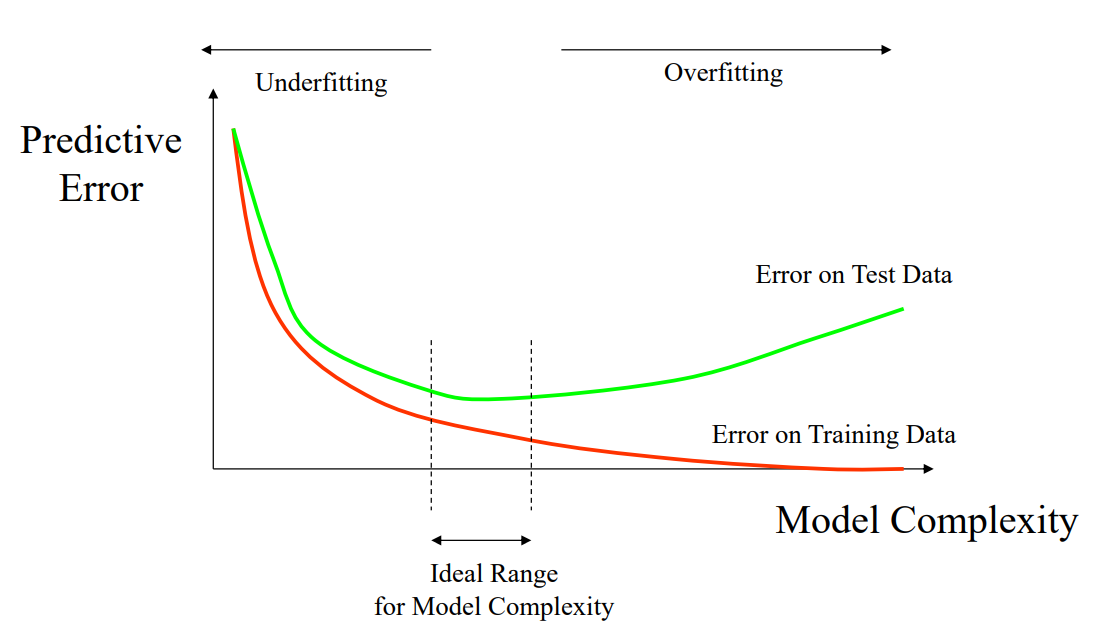
\includegraphics[width=0.7\textwidth]{img/performance evaluation/overfitting_vs_underfitting.png}
    \caption{Rappresentazione dell'overfitting e underfitting}
    \label{fig:overfitting-vs-underfitting}
\end{figure}
Le metriche di valutazione evidenziano tre componenti:
\begin{itemize}
    \item bontà del modello sul train
    \item bontà del modello sul test
    \item complessità del modello (quanti parametri): spazio, tempo in termini
          di $O$
\end{itemize}
Per le metriche sarà fondamentale introdurre la \textbf{matrice di confusione},
in cui:
\begin{equation}
    T[i,j] = \# \ \text{degli esempi etichettati come} \ i \ \text{predetti come
        classe} \ j
\end{equation}
Se si è nel caso di classificazione binaria allora:
\begin{itemize}
    \item $i=0, j=0$, true positive, \textbf{TP}: esempi positivi predetti come
          positivi
    \item $i=0, j=1$, false negative, \textbf{FN}: esempi positivi predetti come
          negativi
    \item $i=1, j=0$, false positive, \textbf{FP}: esempi negativi predetti come
          positivi
    \item $i=1, j=1$, true negative, \textbf{TN}: esempi negativi predetti come
          negativi
\end{itemize}
L'obiettivo sarà quello di massimizzare la diagonale e minimizzare il resto.
\section{Metriche di valutazione}
Le metriche di valutazione sono differenti e si possono calcolare in modo aggregato
su tutte le classi oppure si possono calcolare su una classe alla volta e in un
secondo momento aggregarle secondo delle medie. Generalmente in caso di problemi
di classificazione multi-classe le metriche si calcoleranno sulle singole classi e
si aggregheranno utilizzando diversi metodi.

Le metriche aggregate sono:
\begin{itemize}
    \item \textbf{Tasso di errore}:
          Metrica più naturale che consiste nel calcolo della proporzione degli
          errori su tutto l'insieme di istanze dato in input al modello. Gli errori
          possono essere calcolati secondo lo scarto o secondo le distanze.
    \item \textbf{Accuracy}:
          Misura la proporzione di istanze correttamente classificate su tutto
          l'insieme dato in input sul set.
          \begin{equation}
              Ac = \frac{TP+TN}{TP+TN+FP+FN}
          \end{equation}
    \item \textbf{Precision}:
          La precision misura la proporzione di esempi positivi predetti come
          positivi (TP) sul numero totale di esempi predetti come positivi.
          \begin{equation}
              P=\frac{TP}{TP+FP}
          \end{equation}
    \item \textbf{Recall}:
          La recall misura la proporzione di esempi positivi predetti come positivi
          (TP) sul numero totale di esempi positivi predetti come positivi ed
          esempi positivi predetti come negativi.
          \begin{equation}
              R=\frac{TP}{TP+FN}
          \end{equation}
    \item \textbf{F-measure}:
          La F-measure calcola la media armonica della precision e della recall.
          \begin{equation}
              F = \frac{2\cdot P\cdot R}{P+R}
          \end{equation}
\end{itemize}
Le ultime tre le calcoleremo sulle singole classi:
\begin{itemize}
    \item \textbf{Precision}:
          \begin{equation}
              P(l)=\frac{\# \ \text{di istanze correttamente predette come} \ l}{\#
                  \ \text{di istanze predette come} \ l}
          \end{equation}
    \item \textbf{Recall}:
          \begin{equation}
              R(l)=\frac{\# \ \text{di istanze correttamente predette come} \ l}{\#
                  \ \text{di istanze di classe} \ l}
          \end{equation}
    \item \textbf{F-measure}:
          \begin{equation}
              F(l) = \frac{2\cdot P(l)\cdot R(l)}{P(l)+R(l)}
          \end{equation}
\end{itemize}

Come introdotto precedentemente, si potranno aggregare secondo i seguenti metodi:
\begin{itemize}
    \item \textbf{macro avg}: fa la media della performance tra le diverse classi
          delle singole metriche, utilizzata quando le classi sono di uguale importanza.
          \begin{equation}
              Perf\ast = \frac{1}{|L|}\sum\limits_{l=1}^{|L|} Perf(l), \ Perf \in
              \left\{Ac, P, R, F\right\}
          \end{equation}
    \item \textbf{micro avg}: media pesata della performance rispetto alla cardinalità
          della classe, utilizzata quando le classi sono di diversa importanza.
          \begin{equation}
              Perf\ast = \sum\limits_{l=1}^{|L|} \frac{|class(l)|}{\text{tot.
                      istanze}}Perf(l), \ Perf \in \left\{Ac, P, R, F\right\}
          \end{equation}
          (possiamo anche specificare un peso a piacere l'importante che si
          garantisca il range della metrica)
\end{itemize}
Il confronto dei modelli si può effettuare utilizzando le \textbf{curve ROC} che
mettono a confronto $TP rate$ e $FP rate$. La curva ROC non sono altro che la
valutazione del modello con diverse soglie decisionali da $0$ a $1$.
\begin{definizione}
    La \textbf{soglia decisionale} di un modello è il parametro di confidenza
    che specifica se classificare l'esempio secondo una classe oppure un'altra.
\end{definizione}
\begin{esempio}
    Per esempio nell'algoritmo di Bayes la soglia decisionale è quella che permette
    di specificare sopra che probabilità classificare l'esempio come $T$. Di default
    è $0.5$.
\end{esempio}
Modificando la soglia del modello si possono avere diversi comportamenti:
\begin{itemize}
    \item $\theta \to 1$: il modello è più conservativo quindi si migliorerà la
          precision, peggiorando la recall.
    \item $\theta \to 0$: il modello è meno conservativo, tendendo a classificare
          quindi più facilmente come $T$, quindi migliorerà la
          recall, ma si peggiorerà la precision.
\end{itemize}
La \textbf{curva ROC} si costruisce eseguendo i modelli con treshold diverse
incrementali, al termine dell'esecuzione si ricalcola la \textbf{matrice di
    confusione}, per ottenere i nuovi $TPR$ e $FPR$ da utilizzare per disegnare
il punto sulla curva associato alla soglia settata inizialmente.

Per effettuare il confronto tra modelli, disegneremo nello stesso grafico le
\textbf{curve ROC} associate, permettendoci di studiare il comportamento di ciascun
modello. Generalmente si aggiungono al confronto anche \text{classificatore
    perfetto} (curva verde) e quello \textbf{randomico} (curva rossa). Si definirà
il modello migliore quello che ha la curva dominante rispetto alle altre. Quando
le curve sono simili e si intersecano, allora si deve studiare l'area sottesa
alla curva chiamata \textbf{area AUC}, calcolabile facilmente utilizzando le librerie.
\begin{figure}[!ht]
    \centering
    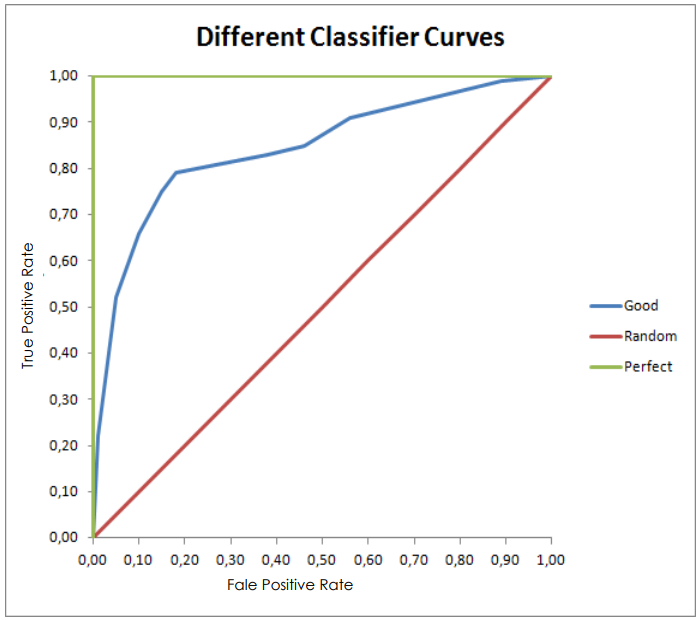
\includegraphics[width=0.7\textwidth]{img/performance evaluation/curva-di-ROC.png}
    \caption{Esempio di curva di ROC}
    \label{fig:curva-di-ROC}
\end{figure}
Confrontando secondo la metrica dell'area AUC, il modello
migliore è quello con la curva con AUC maggiore. L'AUC è utile per:
\begin{itemize}
    \item \textbf{training model}: compara l'apprendimento dei modelli diversi
          sullo stesso training
    \item \textbf{training e production}: specifica una valutazione delle performance
          del modello facendo variare la treshold.
\end{itemize}
La metrica AUC ha delle limitazioni:
\begin{itemize}
    \item perde di significato quando si hanno classi di diversa importanza
    \item quando le classi del dataset sono molto sbilanciate può essere sensibile
          perché una classe sarà predominante nel calcolo della metrica rispetto alle
          altre
\end{itemize}
Un altro modo per valutare il modello sono le \textbf{Curve di apprendimento},
sono delle curve che dicono, al variare della numerosità del campione, come si
comporta il modello in termini di accuratezza. In sostanza si traina il modello
su tutte le combinazioni del dataset di dimensione fissata, si calcola l'accuratezza,
alla fine si computa la media (corrisponde al punto rosso) e si calcola la varianza
(rappresentata dalle barre blu). Successivamente, si reitera il procedimento aumentando
la dimensione del campione. Le curve specificano quanti dati sono necessari per
la fase di training, per avere un modello con performance accettabili in termini
di tempo di apprendimento e della performance. Il calcolo della curva è molto
pesante ma spesso si costruisce parzialmente.
\begin{figure}[!ht]
    \centering
    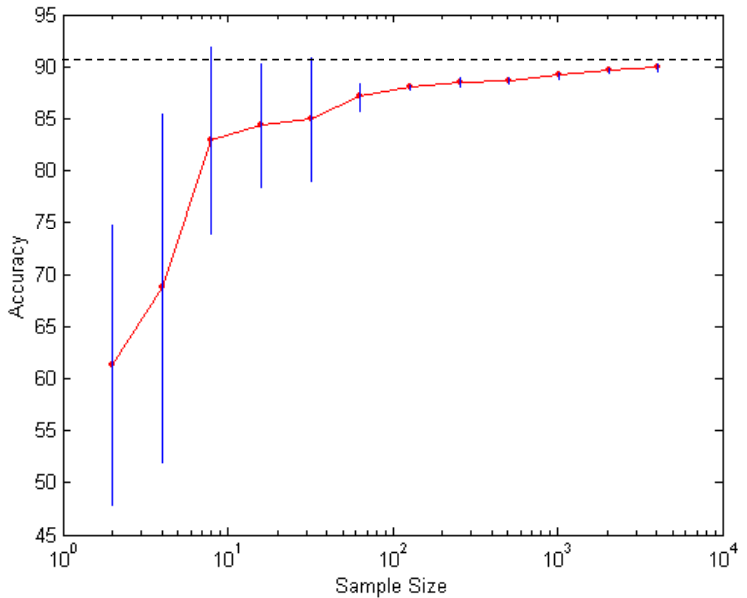
\includegraphics[width=0.7\textwidth]{img/performance evaluation/curva-di-apprendimento.png}
    \caption{Esempio di curva di apprendimento}
    \label{fig:curva-di-apprendimento}
\end{figure}
\section{Valutazione del modello rispetto alla dimensionalità del dataset}
La dimensionalità del dataset è importante per la valutazione del modello, innanzitutto
bisogna identificare quando un dataset è di grandi dimensioni:
\begin{itemize}
    \item \textbf{dataset di grandi dimensioni}: quando il dataset contiene almeno
          $10000$ istanze
    \item \textbf{dataset di medie dimensioni}: quando il dataset contiene tra
          $100$ e $10000$ istanze
    \item \textbf{dataset di piccole dimensioni}: quando il dataset è di dimensione
          molto piccola, $<100$ istanze
\end{itemize}
La valutazione del modello su un dataset di grandi dimensioni può essere fatta
effettuando la suddivisione tra  $80\%$ train set e $20\%$ test randomicamente.
Si allenerà il classificatore sul train set e si valuta sul test set.

\begin{figure}[!ht]
    \centering
    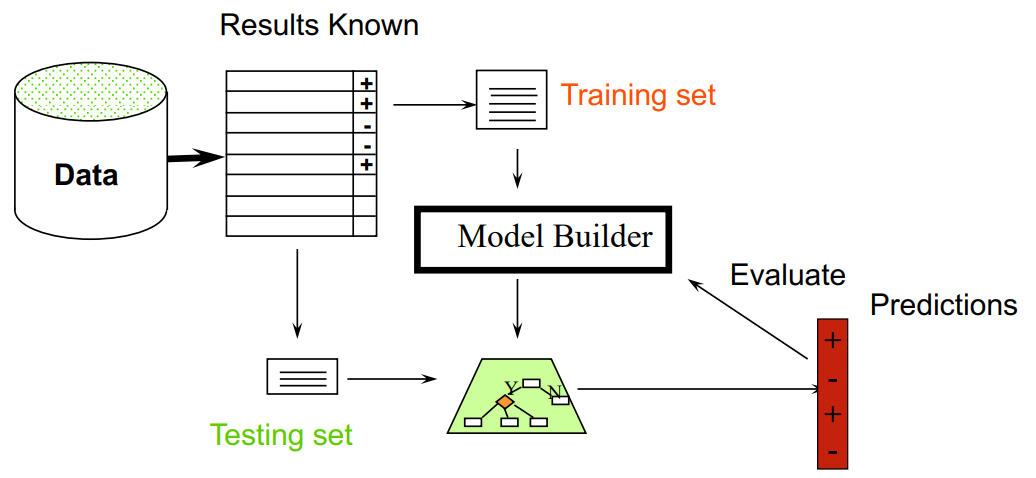
\includegraphics[width=0.7\textwidth]{img/performance evaluation/eval-big-dataset.png}
    \caption{Schema di valutazione di un modello su un dataset di grosse dimensioni}
    \label{fig:eval-big-dataset}
\end{figure}

Ricorda sempre che i dati di test non devono mai essere usati per il train e nemmeno
per il tuning degli iperparametri. Per effettuare il tuning degli iperparametri allora
si partizionerà il train set in training e validation, in modo da calcolare le
metriche sul validation per tunnare gli iperparametri. Per la valutazione del modello
finale si userà sempre il test set.

\begin{figure}[!ht]
    \centering
    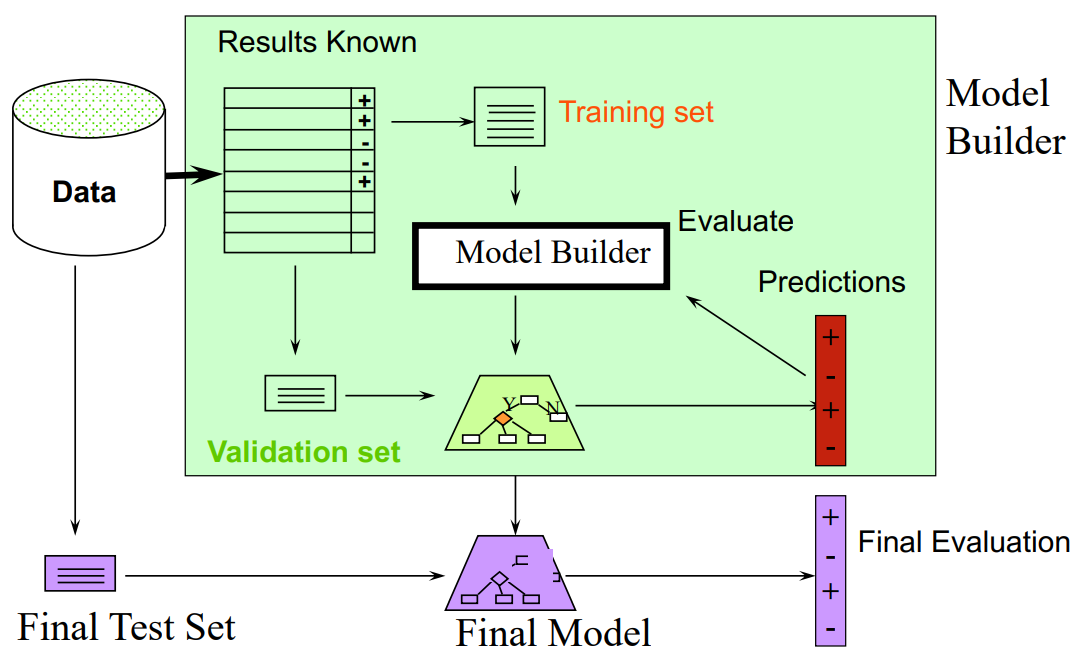
\includegraphics[width=0.7\textwidth]{img/performance evaluation/eval-big-dataset-train-validation-test.png}
    \caption{Schema di valutazione di un modello su un dataset di grosse dimensioni
        con suddivisione train-validation-test}
    \label{fig:eval-big-dataset-train-validation-test}
\end{figure}

Per valutare il modello su un dataset di piccole dimensioni non si effettua più
la suddivisione training, validation e test set, perché i dati sono pochissimi non
avremo una rappresentazione coerente della distribuzione dei dati. La soluzione è
quella di utilizzare \textbf{repeated holdout}, ovvero effettuare la valutazione
del modello allenandolo in più interazioni su una suddivisione dei dati che cambia
ogni volta, stando attenti che in una iterazioni i sottoinsiemi di train e test siano
disgiunti. Ad ogni iterazione si valuta il modello e alla fine si ha la valutazione
finale aggregando le valutazioni delle singole iterazioni.

Questo ragionamento si può applicare su dataset di dimensioni medie sfruttando la
\textbf{k-fold cross-validation} che consiste del suddividere i dati in $k$
sottoinsiemi di uguale dimensione e considerare la maggior parte dei $k$ sottoinsiemi
come train mentre i rimanenti come test. Con questa suddivisione si esegue il modello
iterandolo più volte su questa suddivisione cambiando ogni volta i sottoinsiemi
dedicati al test set e quelli dedicati al train, ci si fermerà una volta
che sono stati testati tutte le combinazioni dei test set. La valutazione finale
sarà l'aggregazione delle valutazioni ad ogni iterazione. Generalmente si utilizza
$\text{stratified} \ 10 \ \text{-fold cross-validation}$ ovvero si ha $k=10$ sottoinsiemi
in cui per ciascun sottoinsieme si cerca di mantenere la stessa distribuzione delle
classi presente nel dataset, in questo modo si riesce a stimare meglio la valutazione
e si diminuisce la varianza della stima, in aggiunta, le iterazioni saranno $10$.

Per i dataset molto piccoli si usano \textbf{leave-one-out}, uguale al k-fold
cross-validation con la differenza che il test sarà composto da un unico elemento,
mentre il train sarà composto da tutti gli altri elementi del dataset. Si ripete
la valutazione del modello fino a quando tutti gli elementi sono stati utilizzati
come test. In questo modo si riesce ad utilizzare molto bene i dati, ma è molto
costoso.

Infine, se il modello deve essere messo in produzione, allora, una volta trovato
il modello migliore, effettuo il training sull'intero dataset senza effettuare la
partizione.
\section{Affidabilità delle misure di performance}
Per avere maggior affidabilità sul confronto tra le misure della performance, non ci
si può solo basare sulla media o sulla varianza della misura, perché sono incomplete.
Il metodo migliore è quello di stimare gli intervalli di confidenza perché:
\begin{itemize}
    \item si capisce la posizione della media
    \item ci da la robustezza determinata dall'ampiezza dell'intervallo di confidenza
\end{itemize}
Dati due modelli con la stessa media, ma uno ha un'ampiezza dell'intervallo minore,
allora quello è il migliore. Se gli intervalli non si sovrappongono e hanno la
stessa ampiezza, allora si prende quello con media migliore.

Un altro approccio di confronto tra modelli consiste nell'utilizzare il test statistico
di significatività che specifica con una certa confidenza, quanto è significativa
la differenza ottenuta:
\begin{itemize}
    \item \textbf{ipotesi nulla}: non esiste una reale differenza
    \item \textbf{ipotesi alternativa}: esiste una reale differenza
\end{itemize}
Il test specifica con che confidenza possiamo rigettare l'ipotesi nulla.
Il test si divide in:
\begin{itemize}
    \item \textbf{test paired}: quando entrambi i modelli hanno imparato nello
          stesso modo sugli stessi dati
    \item \textbf{test unpaired}: altrimenti
\end{itemize}
In generale possiamo dire che:
\begin{itemize}
    \item non guardare solo le performance
    \item considera sempre la complessità
    \item controlla anche l'output
\end{itemize}